\newpage

\section{Moments d'une distribution}

\subsection{Définitions fondamentales des moments}

Après avoir défini l'espérance ($\mu$) et la variance ($\sigma^2$), qui sont les moments d'ordre 1 et 2, nous pouvons généraliser cette idée pour capturer des informations plus subtiles sur la forme d'une distribution.

\begin{definitionbox}[Types de Moments]
Soit $X$ une variable aléatoire ayant une espérance $\mu$ et une variance $\sigma^2$. Pour tout entier positif $m$, on définit les moments suivants :
\begin{itemize}
    \item \textbf{$m$-ième moment (non centré)} : $E[X^m]$.
    \item \textbf{$m$-ième moment centré} : $E[(X - \mu)^m]$.
    \item \textbf{$m$-ième moment standardisé} : $E\left[\left(\frac{X - \mu}{\sigma}\right)^m\right]$.
\end{itemize}
Les moments centrés et standardisés permettent d'étudier les propriétés de la distribution indépendamment de sa position ($\mu$) et de son échelle ($\sigma$).
\end{definitionbox}

\subsection{Asymétrie (Skewness)}

Le premier moment nous donne la tendance centrale. Le deuxième moment (la variance) nous donne la dispersion. Le troisième moment, lui, va nous renseigner sur la \textit{symétrie} de la distribution.

\begin{definitionbox}[Asymétrie (Skewness)]
L'\textbf{asymétrie} (ou \textit{skewness}) d'une variable aléatoire $X$ de moyenne $\mu$ et d'écart-type $\sigma$ est définie comme le \textbf{troisième moment standardisé} :
$$ \text{Skew}(X) = E\left[ \left( \frac{X - \mu}{\sigma} \right)^3 \right]. $$
\end{definitionbox}

\begin{intuitionbox}[Comprendre la Formule du Skewness]
Pour une variable aléatoire $X$ de moyenne $\mu$ et d'écart-type $\sigma$, le \textbf{skewness} est défini comme :
\[
\text{Skew}(X) = \frac{E[(X - \mu)^3]}{\sigma^3}
\]

\medskip

\textbf{Logique du numérateur : le moment centré d'ordre 3}
\begin{itemize}
    \item Le terme $(X - \mu)^3$ est le \textbf{cube de l'écart à la moyenne}
    \item Contrairement à $(X - \mu)^2$ (toujours positif), le cube \textbf{conserve le signe} de l'écart
    \item Il pondère différemment les observations à gauche et à droite de la moyenne
\end{itemize}

\medskip

% --- MODIFIÉ : Tableau supprimé et fusionné dans la liste ---
\textbf{Interprétation intuitive}
\begin{itemize}
    \item \textbf{Skewness = 0 (Symétrique)} : La distribution est symétrique. Les écarts positifs et négatifs s'annulent. Typiquement : Moyenne = Médiane = Mode.
    \item \textbf{Skewness > 0 (Queue à droite)} : La distribution présente une queue longue à droite. Les grandes valeurs positives sont amplifiées par le cube. Les valeurs extrêmes tirent la moyenne vers la droite.
    \item \textbf{Skewness < 0 (Queue à gauche)} : La distribution présente une queue longue à gauche. Les écarts négatifs dominent. Les valeurs extrêmes tirent la moyenne vers la gauche.
\end{itemize}
% --- FIN MODIFICATION ---

\medskip

\textbf{Pourquoi $\sigma^3$ au dénominateur ?}
\begin{itemize}
    \item Le moment d'ordre 3 est homogène à des unités au cube
    \item On divise par $\sigma^3$ pour obtenir un coefficient \textbf{sans dimension}
    \item Permet la comparaison entre distributions de différentes échelles
\end{itemize}
\end{intuitionbox}

\begin{remarquebox}[Pourquoi Standardiser ?]
En standardisant d'abord ($\frac{X-\mu}{\sigma}$), la définition de $\text{Skew}(X)$ ne dépend ni de la position ($\mu$) ni de l'échelle ($\sigma$) de la distribution, ce qui est raisonnable puisque ces informations sont déjà fournies par la moyenne et l'écart-type. De plus, cette standardisation garantit que l'asymétrie est invariante par changement d'unité de mesure (par exemple, passer des pouces aux mètres n'affecte pas la valeur de l'asymétrie).
\end{remarquebox}

\subsection{Propriétés de symétrie}

Le skewness est une mesure numérique de l'asymétrie. Mais nous pouvons aussi définir la symétrie de manière formelle.

\begin{definitionbox}[Symétrie d'une Variable Aléatoire]
On dit qu'une variable aléatoire $X$ a une distribution \textbf{symétrique} autour de $\mu$ si la variable $X - \mu$ a la même distribution que $\mu - X$. On dit aussi que $X$ est symétrique ou que sa distribution est symétrique. Ces trois formulations ont le même sens.
\end{definitionbox}

\begin{theorembox}[Symétrie en Termes de Fonction de Densité]
Soit $X$ une variable aléatoire continue de fonction de densité de probabilité (PDF) $f$. Alors, $X$ est symétrique autour de $\mu$ si et seulement si :
$$ f(x) = f(2\mu - x) \quad \text{pour tout } x. $$
\end{theorembox}

\begin{proofbox}[Preuve du Théorème de Symétrie]
Soit $F$ la fonction de répartition (CDF) de $X$. Si la symétrie tient, alors :
$$ F(x) = P(X \le x) = P(X - \mu \le x - \mu) = P(\mu - X \le x - \mu) = P(X \ge 2\mu - x) = 1 - F(2\mu - x). $$

En prenant la dérivée des deux côtés par rapport à $x$, on obtient :
$$ f(x) = \frac{d}{dx}F(x) = \frac{d}{dx}[1 - F(2\mu - x)] = f(2\mu - x). $$

Cela démontre que la condition $f(x) = f(2\mu - x)$ est nécessaire et suffisante pour la symétrie.
\end{proofbox}

\subsection{Aplatissement (Kurtosis)}

Après l'asymétrie (ordre 3), le moment d'ordre 4 nous informe sur "l'épaisseur" des queues de la distribution, c'est-à-dire la probabilité d'obtenir des valeurs très éloignées de la moyenne.

\begin{definitionbox}[Kurtosis (Aplatissement)]
Pour une variable aléatoire $X$ de moyenne $\mu$ et d'écart-type $\sigma$, le \textbf{kurtosis} est défini comme le \textbf{quatrième moment standardisé} :
$$ \text{Kurtosis}(X) = E\left[ \left( \frac{X - \mu}{\sigma} \right)^4 \right]. $$

Dans la pratique, on utilise plus souvent le \textbf{kurtosis excessif} (ou excès de kurtosis), défini comme :
$$ \text{Excess Kurtosis}(X) = E\left[ \left( \frac{X - \mu}{\sigma} \right)^4 \right] - 3. $$
La soustraction de 3 fait en sorte que le kurtosis d'une loi normale soit égal à 0.
\end{definitionbox}

\begin{intuitionbox}[Comprendre la Kurtosis]
Pour une variable aléatoire $X$, le \textbf{kurtosis} est défini comme :
\[
\text{Kurt}(X) = \frac{E[(X - \mu)^4]}{\sigma^4}
\]
et l'\textbf{excess kurtosis} (kurtosis excédentaire) comme : $\text{Excess Kurtosis} = \text{Kurt}(X) - 3$.

\medskip

\textbf{Pourquoi le moment d'ordre 4 ?}
\begin{itemize}
    \item Comme la variance, on utilise une puissance paire (pas d'effet de signe)
    \item La puissance 4 \textbf{amplifie énormément les écarts extrêmes}
    \item Mesure le \textbf{poids des queues} et la \textbf{concentration autour de la moyenne}
\end{itemize}

\medskip

% --- MODIFIÉ : Tableau supprimé et fusionné dans la liste ---
\textbf{Interprétation intuitive (basée sur l'Excess Kurtosis)}
\begin{itemize}
    \item \textbf{Leptokurtique (Excess Kurtosis > 0)} : Kurtosis total > 3. Distribution pointue avec des queues épaisses. Les événements extrêmes sont plus probables que pour une loi normale.
    \item \textbf{Mésocurtique (Excess Kurtosis = 0)} : Kurtosis total = 3. C'est la référence (loi normale).
    \item \textbf{Platykurtique (Excess Kurtosis < 0)} : Kurtosis total < 3. Distribution aplatie avec des queues légères et un centre large. Les événements extrêmes sont moins probables.
\end{itemize}
% --- FIN MODIFICATION ---

\medskip

\textbf{Application en finance}
\begin{itemize}
    \item Les rendements financiers ont souvent un excès de kurtosis positif
    \item Indique une probabilité plus élevée d'événements extrêmes que la loi normale
    \item Justifie le "vol smile" dans les options
\end{itemize}

\medskip

\textbf{Pourquoi $\sigma^4$ au dénominateur ?}
\begin{itemize}
    \item Le moment d'ordre 4 est homogène à des unités$^4$
    \item On divise par $\sigma^4$ pour un coefficient \textbf{sans dimension}
\end{itemize}
\end{intuitionbox}

\subsection{Exemples de distributions}

Pour bien fixer les idées, comparons le skewness et le kurtosis de plusieurs distributions classiques. Notez que dans les graphiques suivants, le "Kurtosis" affiché est l'\textit{excess kurtosis} (centré à 0).

\begin{examplebox}[La Distribution Normale (Mésokurtique)]

\begin{center}
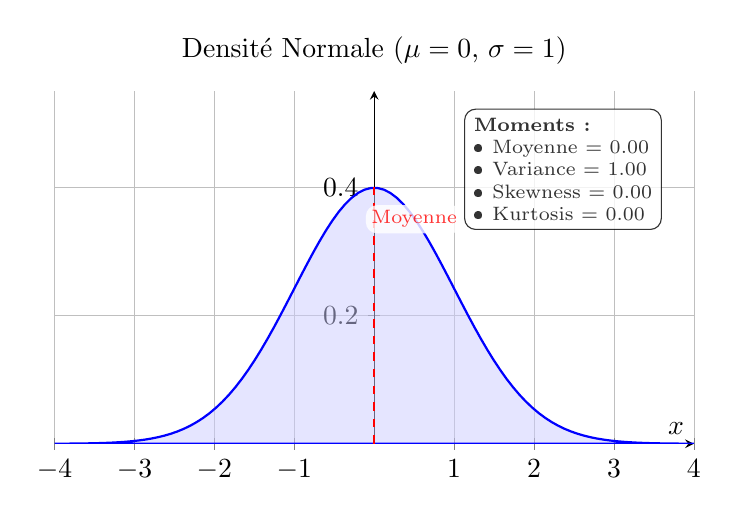
\begin{tikzpicture}
  \begin{axis}[
    width=0.8\textwidth,
    height=0.5\textwidth,
    xlabel={$x$},
    title={Densité Normale ($\mu=0$, $\sigma=1$)},
    grid=both,
    grid style={line width=.1pt, draw=gray!30},
    major grid style={line width=.2pt,draw=gray!50},
    domain=-4:4,
    samples=100,
    enlargelimits=false,
    axis lines=middle,
    xmin=-4, xmax=4,
    ymin=0, ymax=0.55
  ]
 
  % Courbe de densité
  \addplot [thick, color=blue, fill=blue!20, fill opacity=0.5] 
    {1/(sqrt(2*pi))*exp(-x^2/2)} \closedcycle;
 
  % Ligne de la moyenne
  \addplot [red, dashed, thick] coordinates {(0,0) (0,0.4)};
  \node[red, fill=white, font=\scriptsize, rounded corners, inner sep=2pt, opacity=0.8] at (axis cs:0.5,0.35) {Moyenne};
 
  % Boîte de texte avec moments seulement
  \node [draw=black, fill=white, rounded corners, font=\scriptsize, align=left, anchor=north east, opacity=0.8] 
    at (axis description cs:0.95,0.95) { % MODIFIÉ
    \textbf{Moments :}\\
    • Moyenne = 0.00\\
    • Variance = 1.00\\
    • Skewness = 0.00\\
    • Kurtosis = 0.00
    };
    
  \end{axis}
\end{tikzpicture}
\end{center}

La distribution normale est l'archétype de la courbe en cloche. Imaginez une cible : la majorité des flèches touchent le centre, et plus on s'éloigne du centre, moins il y a de chances d'être touché. C'est une distribution parfaitement symétrique, ce qui se traduit par un \textbf{skewness nul (0.00)}. Son pic est ni trop pointu, ni trop plat : c'est notre point de référence, on dit qu'elle est \textbf{mésokurtique}, d'où son kurtosis de \textbf{0.00}. C'est la base de nombreuses analyses statistiques car elle modélise naturellement beaucoup de phénomènes.

\end{examplebox}

\begin{examplebox}[La Distribution Exponentielle (Asymétrique à Droite)]

\begin{center}
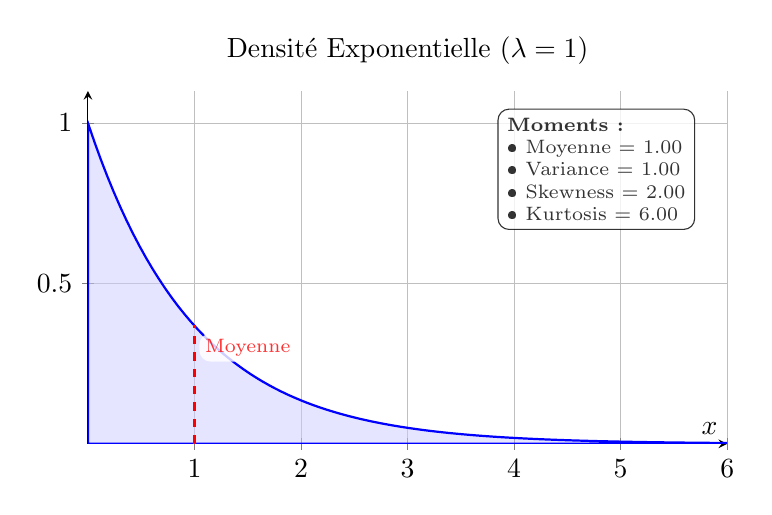
\begin{tikzpicture}
  \begin{axis}[
    width=0.8\textwidth,
    height=0.5\textwidth,
    xlabel={$x$},
    title={Densité Exponentielle ($\lambda=1$)},
    grid=both,
    grid style={line width=.1pt, draw=gray!30},
    major grid style={line width=.2pt,draw=gray!50},
    domain=0:6,
    samples=100,
    enlargelimits=false,
    axis lines=middle,
    xmin=0, xmax=6,
    ymin=0, ymax=1.1
  ]
 
  % Courbe de densité exponentielle
  \addplot [thick, color=blue, fill=blue!20, fill opacity=0.5] 
    {exp(-x)} \closedcycle;
 
  % Ligne de la moyenne
  \addplot [red, dashed, thick] coordinates {(1,0) (1,0.37)};
  \node[red, fill=white, font=\scriptsize, rounded corners, inner sep=2pt, opacity=0.8] at (axis cs:1.5,0.3) {Moyenne};
 
  % Boîte de texte avec moments seulement
  \node [draw=black, fill=white, rounded corners, font=\scriptsize, align=left, anchor=north east, opacity=0.8] 
    at (axis description cs:0.95,0.95) { % MODIFIÉ
    \textbf{Moments :}\\
    • Moyenne = 1.00\\
    • Variance = 1.00\\
    • Skewness = 2.00\\
    • Kurtosis = 6.00
    };
    
  \end{axis}
\end{tikzpicture}
\end{center}

Imaginez le temps d'attente avant un événement rare, comme un appel téléphonique. La plupart du temps, l'appel arrive vite, mais il peut parfois y avoir de longues attentes. C'est exactement ce que modélise la distribution exponentielle : un pic à gauche et une longue queue à droite. Cela se traduit par un \textbf{skewness positif élevé (2.00)}, indiquant une asymétrie marquée. Elle est aussi \textbf{leptokurtique} (\textbf{kurtosis = 6.00}) : son pic est pointu, et la longue queue droite signifie qu'il y a une probabilité non négligeable de valeurs extrêmes.

\end{examplebox}

\begin{examplebox}[La Distribution Uniforme (Platykurtique)]

\begin{center}
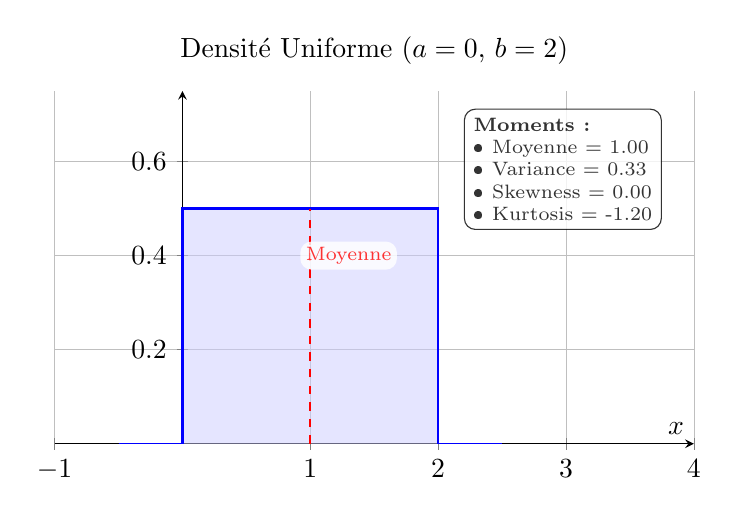
\begin{tikzpicture}
  \begin{axis}[
    width=0.8\textwidth,
    height=0.5\textwidth,
    xlabel={$x$},
    title={Densité Uniforme ($a=0$, $b=2$)},
    grid=both,
    grid style={line width=.1pt, draw=gray!30},
    major grid style={line width=.2pt,draw=gray!50},
    domain=-0.5:2.5,
    samples=100,
    enlargelimits=false,
    axis lines=middle,
    ymin=0,
    ymax=.75,
    xmin=-1, xmax=4
  ]
 
  % Courbe de densité uniforme
  \addplot [thick, color=blue, fill=blue!20, fill opacity=0.5, const plot] 
    coordinates {(-0.5,0) (0,0) (0,0.5) (2,0.5) (2,0) (2.5,0)};
 
  % Ligne de la moyenne
  \addplot [red, dashed, thick] coordinates {(1,0) (1,0.5)};
  \node[red, fill=white, font=\scriptsize, rounded corners, inner sep=2pt, opacity=0.8] at (axis cs:1.3,0.4) {Moyenne};
 
  % Boîte de texte avec moments seulement
  \node [draw=black, fill=white, rounded corners, font=\scriptsize, align=left, anchor=north east, opacity=0.8] 
    at (axis description cs:0.95,0.95) { % MODIFIÉ
    \textbf{Moments :}\\
    • Moyenne = 1.00\\
    • Variance = 0.33\\
    • Skewness = 0.00\\
    • Kurtosis = -1.20
    };
    
  \end{axis}
\end{tikzpicture}
\end{center}

La distribution uniforme, c'est le "tirage au sort parfait" : chaque valeur sur un intervalle a la même chance d'être tirée. Visuellement, c'est un rectangle, donc aucune valeur n'est privilégiée. Elle est symétrique (\textbf{skewness = 0.00}), mais contrairement à la normale, elle est "plate", sans pic central. Cela se traduit par un \textbf{kurtosis négatif (-1.20)}, ce qui signifie qu'elle est \textbf{platykurtique}. Elle est donc très différente des distributions avec un pic central comme la normale.

\end{examplebox}

\begin{examplebox}[La Distribution Log-Normale (Fortement Leptokurtique)]

\begin{center}
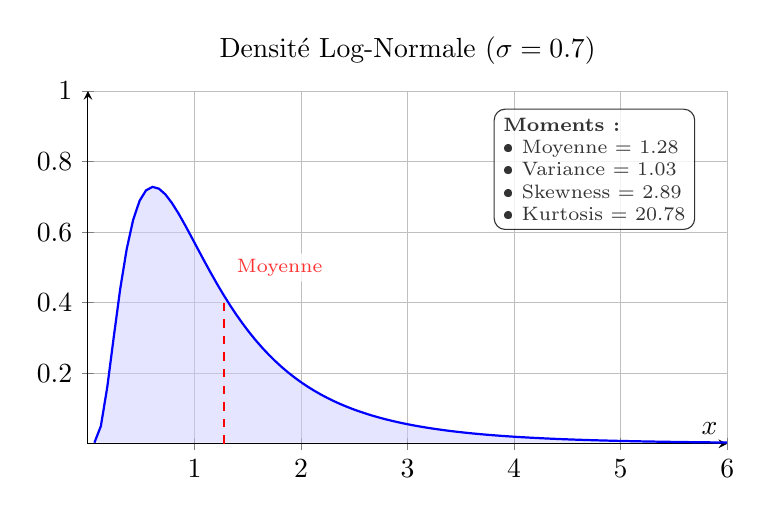
\begin{tikzpicture}
  \begin{axis}[
    width=0.8\textwidth,
    height=0.5\textwidth,
    xlabel={$x$},
    title={Densité Log-Normale ($\sigma=0.7$)},
    grid=both,
    grid style={line width=.1pt, draw=gray!30},
    major grid style={line width=.2pt,draw=gray!50},
    domain=0:6,
    samples=100,
    enlargelimits=false,
    axis lines=middle,
    xmin=0, xmax=6,
    ymin=0, ymax=1
  ]
 
  % Courbe de densité log-normale
  \addplot [thick, color=blue, fill=blue!20, fill opacity=0.5] 
    {1/(x*0.7*sqrt(2*pi))*exp(-(ln(x))^2/(2*0.7^2))};
 
  % Ligne de la moyenne
  \addplot [red, dashed, thick] coordinates {(1.28,0) (1.28,0.4)};
  \node[red, fill=white, font=\scriptsize, rounded corners, inner sep=2pt, opacity=0.8] at (axis cs:1.8,0.5) {Moyenne};
 
  % Boîte de texte avec moments seulement
  \node [draw=black, fill=white, rounded corners, font=\scriptsize, align=left, anchor=north east, opacity=0.8] 
    at (axis description cs:0.95,0.95) { % MODIFIÉ
    \textbf{Moments :}\\
    • Moyenne = 1.28\\
    • Variance = 1.03\\
    • Skewness = 2.89\\
    • Kurtosis = 20.78
    };
    
  \end{axis}
\end{tikzpicture}
\end{center}

La log-normale est une distribution très asymétrique. Imaginez la richesse d'une population : la majorité est modeste, mais il existe une petite proportion de très riches, ce qui "étire" la droite de la courbe. Cela donne un \textbf{skewness très élevé (2.89)}. Elle est extrêmement \textbf{leptokurtique} (\textbf{kurtosis = 20.78}) : un pic très aigu et une queue droite très lourde. Cela signifie qu'il y a un risque élevé de valeurs extrêmement grandes, ce qui la rend très utile pour modéliser des phénomènes avec de rares événements extrêmes.

\end{examplebox}


\subsection{Exercices}

% --- Définitions Fondamentales des Moments ---

\begin{exercicebox}[Exercice 1 : Associer les Moments]
Associez chaque description au moment correspondant :
\begin{enumerate}
    \item $E[X]$
    \item $\sqrt{E[(X-\mu)^2]}$
    \item $E[(X-\mu)^2]$
    \item $E[\left(\frac{X-\mu}{\sigma}\right)^3]$
    \item $E[\left(\frac{X-\mu}{\sigma}\right)^4] - 3$
\end{enumerate}

\textbf{Termes :} Variance, Asymétrie (Skewness), Espérance (Moyenne), Écart-type, Excès de Kurtosis.
\end{exercicebox}

\begin{exercicebox}[Exercice 2 : Calcul des Moments Centrés]
Soit $X$ une v.a. avec $\mu = 2$. La PMF de $X$ est :
$P(X=0)=0.2$, $P(X=2)=0.6$, $P(X=4)=0.2$.
\begin{enumerate}
    \item Vérifiez que $E[X] = 2$.
    \item Calculez le 2ème moment centré, $E[(X-\mu)^2]$ (la Variance).
    \item Calculez le 3ème moment centré, $E[(X-\mu)^3]$.
\end{enumerate}
\end{exercicebox}

\begin{exercicebox}[Exercice 3 : Calcul des Moments Standardisés]
En utilisant la v.a. $X$ de l'exercice 2 (avec $\mu=2$ et $\text{Var}(X) = 1.6$) :
\begin{enumerate}
    \item Calculez le Skewness, $\text{Skew}(X)$.
    \item Que pouvez-vous conclure sur la symétrie de cette distribution ?
\end{enumerate}
(Rappel : $\sigma = \sqrt{1.6} \approx 1.265$).
\end{exercicebox}

% --- Asymétrie (Skewness) ---

\begin{exercicebox}[Exercice 4 : Interprétation Visuelle du Skewness]
Pour chacune des distributions décrites, indiquez si le skewness est \textbf{positif (> 0)}, \textbf{négatif (< 0)} ou \textbf{nul (= 0)}.
\begin{enumerate}
    \item La distribution $\text{Exp}(\lambda)$ (queue longue à droite).
    \item Une distribution où Moyenne = 10, Médiane = 12, Mode = 13 (queue longue à gauche).
    \item La distribution $\mathcal{N}(\mu, \sigma^2)$.
    \item La distribution des revenus dans un pays (beaucoup de salaires bas, quelques salaires très élevés).
\end{enumerate}
\end{exercicebox}

\begin{exercicebox}[Exercice 5 : Skewness d'une Distribution Simple]
Soit $X$ une v.a. : $P(X=0)=0.1$, $P(X=1)=0.8$, $P(X=10)=0.1$.
\begin{enumerate}
    \item Calculez $\mu = E[X]$.
    \item Calculez $\sigma^2 = \text{Var}(X)$.
    \item Calculez $E[(X-\mu)^3]$.
    \item Le skewness est-il positif, négatif ou nul ? (Le calcul complet n'est pas nécessaire si vous justifiez).
\end{enumerate}
\end{exercicebox}

\begin{exercicebox}[Exercice 6 : Skewness d'une Variable de Bernoulli]
Soit $X \sim \text{Bern}(p)$. On rappelle que $\mu = p$ et $\sigma^2 = p(1-p)$.
\begin{enumerate}
    \item Calculez $E[X^3]$. (Indice : $X^3 = X$).
    \item Calculez le 3ème moment centré $E[(X-p)^3]$ en développant l'expression.
    \item Calculez le skewness $\text{Skew}(X) = \frac{E[(X-p)^3]}{\sigma^3}$.
    \item Pour quelle valeur de $p$ cette distribution est-elle symétrique ?
\end{enumerate}
\end{exercicebox}

% --- Symétrie ---

\begin{exercicebox}[Exercice 7 : Définition de la Symétrie]
Soit $X \sim \text{Unif}(-5, 5)$.
\begin{enumerate}
    \item Autour de quel point $\mu$ cette distribution est-elle symétrique ?
    \item Montrez que $f(x) = f(2\mu - x)$ en utilisant la PDF de la loi uniforme.
\end{enumerate}
\end{exercicebox}

\begin{exercicebox}[Exercice 8 : Symétrie et Moments Centrés]
Soit $X$ une v.a. symétrique autour de sa moyenne $\mu$.
Montrez que tous ses moments centrés d'ordre impair sont nuls, c'est-à-dire $E[(X-\mu)^k] = 0$ pour $k=1, 3, 5, \dots$
(Indice : Soit $Y = X-\mu$. $Y$ est symétrique autour de 0. Que vaut $E[Y^k]$ ?).
\end{exercicebox}

\begin{exercicebox}[Exercice 9 : Symétrie de la Loi Normale]
Soit $X \sim \mathcal{N}(\mu, \sigma^2)$.
\begin{enumerate}
    \item La distribution est-elle symétrique ?
    \item Que vaut $\text{Skew}(X)$ ? (Sans calcul, en utilisant le résultat de l'exercice 8).
\end{enumerate}
\end{exercicebox}

\begin{exercicebox}[Exercice 10 : Symétrie et Skewness]
Si $\text{Skew}(X) = 0$, peut-on affirmer que la distribution de $X$ est symétrique ?
(Indice : Pensez à une distribution qui n'est pas symétrique mais où les asymétries se compensent, ex: $P(X=-4)=0.1, P(X=-1)=0.4, P(X=2)=0.5$).
\end{exercicebox}

% --- Aplatissement (Kurtosis) ---

\begin{exercicebox}[Exercice 11 : Interprétation du Kurtosis]
Associez chaque type de distribution à sa description du kurtosis (excédentaire) :
\begin{enumerate}
    \item \textbf{Leptokurtique}
    \item \textbf{Mésokurtique}
    \item \textbf{Platykurtique}
\end{enumerate}

\textbf{Descriptions :}
A. Excès de Kurtosis = 0 (Référence de la loi normale).
B. Excès de Kurtosis < 0 (Distribution "plate" avec des queues fines).
C. Excès de Kurtosis > 0 (Distribution "pointue" avec des queues épaisses).
\end{exercicebox}

\begin{exercicebox}[Exercice 12 : Kurtosis et queues]
Une distribution A a un excès de kurtosis de 5. Une distribution B a un excès de kurtosis de 1.
Laquelle des deux distributions est la plus susceptible de produire des valeurs "extrêmes" (très loin de la moyenne) ?
\end{exercicebox}

\begin{exercicebox}[Exercice 13 : Kurtosis de la Loi Normale]
Soit $Z \sim \mathcal{N}(0, 1)$.
\begin{enumerate}
    \item Que vaut le 4ème moment standardisé $E[Z^4]$ ? (Indice : Pour une $\mathcal{N}(0,1)$, $E[Z^4]=3$).
    \item Que vaut l'excès de kurtosis de $Z$ ?
\end{enumerate}
\end{exercicebox}

\begin{exercicebox}[Exercice 14 : Kurtosis de la Loi Uniforme]
D'après les exemples du cours, la loi $\text{Unif}(a, b)$ a un excès de kurtosis de -1.2.
Est-elle leptokurtique, mésokurtique ou platykurtique ?
\end{exercicebox}

% --- Synthèse et Propriétés ---

\begin{exercicebox}[Exercice 15 : Invariance des Moments Standardisés]
Soit $X$ une v.a. avec $\mu=10$, $\sigma=2$, $\text{Skew}(X) = 0.5$ et $\text{Excess Kurtosis}(X) = 1$.
Soit $Y = 3X + 5$.
\begin{enumerate}
    \item Calculez $E[Y]$ et $\text{Var}(Y)$.
    \item Que vaut $\text{Skew}(Y)$ ?
    \item Que vaut $\text{Excess Kurtosis}(Y)$ ?
\end{enumerate}
(Indice : Les moments standardisés sont invariants par transformation linéaire $aX+b$ avec $a>0$).
\end{exercicebox}

\begin{exercicebox}[Exercice 16 : Moments d'une Distribution Inconnue]
Une v.a. $Z$ a été standardisée ($E[Z]=0, \text{Var}(Z)=1$).
On sait que $E[Z^3] = 0.8$ et $E[Z^4] = 4.5$.
\begin{enumerate}
    \item Calculez le skewness de $Z$.
    \item Calculez l'excès de kurtosis de $Z$.
\end{enumerate}
\end{exercicebox}

\begin{exercicebox}[Exercice 17 : Identifier la Distribution]
Une distribution $X$ est analysée. On trouve :
$\text{Skew}(X) = 0$ et $\text{Excess Kurtosis}(X) = 0$.
Quelle distribution célèbre partage ces deux propriétés ?
\end{exercicebox}

\begin{exercicebox}[Exercice 18 : Identifier la Distribution (2)]
Une distribution $Y$ est analysée. On trouve :
$\text{Skew}(Y) = 2.0$ et $\text{Excess Kurtosis}(Y) = 6.0$.
Quelle distribution vue en cours (et dans les exemples) correspond à ces valeurs ?
\end{exercicebox}

\begin{exercicebox}[Exercice 19 : Moments non centrés vs centrés]
Soit $X$ une v.a. avec $E[X] = \mu$.
Exprimez le 2ème moment centré $E[(X-\mu)^2]$ en fonction des moments non centrés $E[X^2]$ et $E[X]$. (C'est la formule de calcul de la variance).
\end{exercicebox}

\begin{exercicebox}[Exercice 20 : Moments centrés vs non centrés]
Soit $X$ une v.a. avec $E[X] = \mu$.
Exprimez le 3ème moment centré $E[(X-\mu)^3]$ en fonction des moments non centrés ($E[X^3]$, $E[X^2]$, $E[X]$).
(Indice : Développez $(X-\mu)^3 = X^3 - 3X^2\mu + 3X\mu^2 - \mu^3$ et prenez l'espérance).
\end{exercicebox}

\subsection{Corrections des Exercices}

% --- Corrections : Définitions Fondamentales des Moments ---

\begin{correctionbox}[Correction Exercice 1 : Associer les Moments]
1.  $E[X]$ $\rightarrow$ \textbf{Espérance (Moyenne)}
2.  $\sqrt{E[(X-\mu)^2]}$ $\rightarrow$ \textbf{Écart-type}
3.  $E[(X-\mu)^2]$ $\rightarrow$ \textbf{Variance}
4.  $E[\left(\frac{X-\mu}{\sigma}\right)^3]$ $\rightarrow$ \textbf{Asymétrie (Skewness)}
5.  $E[\left(\frac{X-\mu}{\sigma}\right)^4] - 3$ $\rightarrow$ \textbf{Excès de Kurtosis}
\end{correctionbox}

\begin{correctionbox}[Correction Exercice 2 : Calcul des Moments Centrés]
$P(X=0)=0.2$, $P(X=2)=0.6$, $P(X=4)=0.2$.
1.  $E[X] = (0)(0.2) + (2)(0.6) + (4)(0.2) = 0 + 1.2 + 0.8 = 2.0$. $\mu=2$.
2.  Variance = $E[(X-2)^2]$
    $= (0-2)^2(0.2) + (2-2)^2(0.6) + (4-2)^2(0.2)$
    $= (-2)^2(0.2) + (0)^2(0.6) + (2)^2(0.2)$
    $= 4(0.2) + 0 + 4(0.2) = 0.8 + 0.8 = 1.6$.
3.  3ème moment centré = $E[(X-2)^3]$
    $= (0-2)^3(0.2) + (2-2)^3(0.6) + (4-2)^3(0.2)$
    $= (-8)(0.2) + (0)(0.6) + (8)(0.2)$
    $= -1.6 + 0 + 1.6 = 0$.
\end{correctionbox}

\begin{correctionbox}[Correction Exercice 3 : Calcul des Moments Standardisés]
De l'exercice 2, $\mu=2$, $\text{Var}(X) = 1.6$ et $E[(X-\mu)^3] = 0$.
1.  $\text{Skew}(X) = \frac{E[(X-\mu)^3]}{\sigma^3} = \frac{0}{(1.6)^{3/2}} = 0$.
2.  Le skewness est nul. Cela indique que la distribution est symétrique, ce que l'on peut vérifier (les probabilités $P(\mu-2k)$ et $P(\mu+2k)$ sont égales).
\end{correctionbox}

% --- Corrections : Asymétrie (Skewness) ---

\begin{correctionbox}[Correction Exercice 4 : Interprétation Visuelle du Skewness]
1.  \textbf{Positif (> 0)}. La loi exponentielle a une queue longue à droite.
2.  \textbf{Négatif (< 0)}. L'ordre $\text{Moyenne} < \text{Médiane} < \text{Mode}$ est caractéristique d'une queue à gauche.
3.  \textbf{Nul (= 0)}. La loi normale est parfaitement symétrique.
4.  \textbf{Positif (> 0)}. La grande majorité des gens a un revenu bas/moyen, et une petite minorité a un revenu très élevé, créant une queue longue à droite.
\end{correctionbox}

\begin{correctionbox}[Correction Exercice 5 : Skewness d'une Distribution Simple]
$P(X=0)=0.1$, $P(X=1)=0.8$, $P(X=10)=0.1$.
1.  $\mu = E[X] = (0)(0.1) + (1)(0.8) + (10)(0.1) = 0 + 0.8 + 1.0 = 1.8$.
2.  $E[X^2] = (0^2)(0.1) + (1^2)(0.8) + (10^2)(0.1) = 0 + 0.8 + 10 = 10.8$.
    $\sigma^2 = E[X^2] - \mu^2 = 10.8 - (1.8)^2 = 10.8 - 3.24 = 7.56$.
3.  $E[(X-\mu)^3] = (0-1.8)^3(0.1) + (1-1.8)^3(0.8) + (10-1.8)^3(0.1)$
    $= (-5.832)(0.1) + (-0.512)(0.8) + (551.368)(0.1)$
    $= -0.5832 - 0.4096 + 55.1368 = 54.144$.
4.  Puisque $E[(X-\mu)^3] = 54.144 > 0$, le skewness est \textbf{positif}. Cela est dû à la valeur extrême $X=10$ qui tire la distribution vers la droite.
\end{correctionbox}

\begin{correctionbox}[Correction Exercice 6 : Skewness d'une Variable de Bernoulli]
$X \sim \text{Bern}(p)$, $\mu=p$, $\sigma^2=p(1-p)$.
1.  $X$ ne vaut que 0 ou 1, donc $X^3 = X$. $E[X^3] = E[X] = p$.
2.  $E[(X-p)^3] = E[X^3 - 3X^2p + 3Xp^2 - p^3]$
    $= E[X^3] - 3pE[X^2] + 3p^2E[X] - p^3$
    (Car $X^2=X$ et $X^3=X$)
    $= E[X] - 3pE[X] + 3p^2E[X] - p^3$
    $= p - 3p(p) + 3p^2(p) - p^3 = p - 3p^2 + 3p^3 - p^3 = p - 3p^2 + 2p^3$
    $= p(1 - 3p + 2p^2) = p(1-p)(1-2p)$.
3.  $\text{Skew}(X) = \frac{E[(X-p)^3]}{\sigma^3} = \frac{p(1-p)(1-2p)}{[p(1-p)]^{3/2}} = \frac{1-2p}{\sqrt{p(1-p)}}$.
4.  La distribution est symétrique si $\text{Skew}(X) = 0$. Cela se produit si $1-2p = 0$, donc $p=0.5$.
\end{correctionbox}

% --- Corrections : Symétrie ---

\begin{correctionbox}[Correction Exercice 7 : Définition de la Symétrie]
$X \sim \text{Unif}(-5, 5)$.
1.  La moyenne est $\mu = (-5+5)/2 = 0$. La distribution est symétrique autour de $\mu=0$.
2.  On doit montrer $f(x) = f(2\mu - x) = f(-x)$.
    La PDF est $f(x) = 1/10$ si $x \in [-5, 5]$ et $0$ sinon.
    - Si $x \in [-5, 5]$, alors $-x \in [-5, 5]$. $f(x) = 1/10$ et $f(-x) = 1/10$. Ils sont égaux.
    - Si $x > 5$, $f(x) = 0$. Alors $-x < -5$, $f(-x) = 0$. Ils sont égaux.
    La condition est vérifiée pour tout $x$.
\end{correctionbox}

\begin{correctionbox}[Correction Exercice 8 : Symétrie et Moments Centrés]
Soit $Y = X-\mu$. Si $X$ est symétrique autour de $\mu$, $Y$ est symétrique autour de 0. Sa PDF $f_Y(y)$ est paire : $f_Y(y) = f_Y(-y)$.
On veut calculer $E[Y^k] = \int_{-\infty}^{\infty} y^k f_Y(y) dy$ pour $k$ impair.
La fonction $y^k$ est impaire (car $k$ est impair).
La fonction $f_Y(y)$ est paire.
Le produit d'une fonction impaire et d'une fonction paire est une fonction impaire.
L'intégrale d'une fonction impaire sur un intervalle symétrique $(-\infty, \infty)$ est 0.
Donc, $E[(X-\mu)^k] = E[Y^k] = 0$ pour $k=1, 3, 5, \dots$.
\end{correctionbox}

\begin{correctionbox}[Correction Exercice 9 : Symétrie de la Loi Normale]
1.  Oui, la PDF de la loi normale est parfaitement symétrique autour de sa moyenne $\mu$.
2.  Le Skewness est basé sur le 3ème moment centré ($k=3$, qui est impair). D'après l'exercice 8, tous les moments centrés impairs d'une distribution symétrique sont nuls.
    Donc $\text{Skew}(X) = 0$.
\end{correctionbox}

\begin{correctionbox}[Correction Exercice 10 : Symétrie et Skewness]
Non. $\text{Skew}(X)=0$ est une condition nécessaire mais non suffisante pour la symétrie. Une distribution peut avoir un skewness nul tout en n'étant pas symétrique, si les asymétries de gauche et de droite "s'annulent" dans le calcul du 3ème moment.
\end{correctionbox}

% --- Corrections : Aplatissement (Kurtosis) ---

\begin{correctionbox}[Correction Exercice 11 : Interprétation du Kurtosis]
1.  \textbf{Leptokurtique} $\rightarrow$ \textbf{C.} Excès de Kurtosis > 0 (Pointue, queues épaisses).
2.  \textbf{Mésokurtique} $\rightarrow$ \textbf{A.} Excès de Kurtosis = 0 (Référence normale).
3.  \textbf{Platykurtique} $\rightarrow$ \textbf{B.} Excès de Kurtosis < 0 (Plate, queues fines).
\end{correctionbox}

\begin{correctionbox}[Correction Exercice 12 : Kurtosis et queues]
Un excès de kurtosis plus élevé signifie des queues plus épaisses.
La \textbf{Distribution A} (kurtosis=5) est beaucoup plus susceptible de produire des valeurs extrêmes que la Distribution B (kurtosis=1).
\end{correctionbox}

\begin{correctionbox}[Correction Exercice 13 : Kurtosis de la Loi Normale]
$Z \sim \mathcal{N}(0, 1)$.
1.  $E[Z^4]$ est le 4ème moment standardisé. Par définition, c'est le kurtosis (non excessif). Pour la loi normale, $\text{Kurtosis}(Z) = 3$. Donc $E[Z^4] = 3$.
2.  Excès de Kurtosis = $\text{Kurtosis}(Z) - 3 = 3 - 3 = 0$.
\end{correctionbox}

\begin{correctionbox}[Correction Exercice 14 : Kurtosis de la Loi Uniforme]
L'excès de kurtosis est -1.2, ce qui est négatif.
La distribution uniforme est \textbf{platykurtique} (plus "plate" que la normale).
\end{correctionbox}

% --- Corrections : Synthèse et Propriétés ---

\begin{correctionbox}[Correction Exercice 15 : Invariance des Moments Standardisés]
$Y = 3X + 5$.
1.  $E[Y] = 3E[X] + 5 = 3(10) + 5 = 35$.
    $\text{Var}(Y) = 3^2 \text{Var}(X) = 9 (2^2) = 36$.
2.  Le skewness est invariant par transformation linéaire affine (si $a>0$). $\text{Skew}(Y) = \text{Skew}(X) = 0.5$.
3.  L'excès de kurtosis est invariant par transformation linéaire affine. $\text{Excess Kurtosis}(Y) = \text{Excess Kurtosis}(X) = 1$.
\end{correctionbox}

\begin{correctionbox}[Correction Exercice 16 : Moments d'une Distribution Inconnue]
$Z$ est déjà standardisée ($\mu=0, \sigma=1$).
1.  $\text{Skew}(Z) = E\left[ \left( \frac{Z - 0}{1} \right)^3 \right] = E[Z^3] = 0.8$.
2.  $\text{Excess Kurtosis}(Z) = E\left[ \left( \frac{Z - 0}{1} \right)^4 \right] - 3 = E[Z^4] - 3 = 4.5 - 3 = 1.5$.
\end{correctionbox}

\begin{correctionbox}[Correction Exercice 17 : Identifier la Distribution]
La \textbf{Loi Normale} $\mathcal{N}(\mu, \sigma^2)$ est la distribution de référence qui est symétrique ($\text{Skew}=0$) et mésokurtique ($\text{Excess Kurtosis}=0$).
\end{correctionbox}

\begin{correctionbox}[Correction Exercice 18 : Identifier la Distribution (2)]
La \textbf{Loi Exponentielle} $\text{Exp}(\lambda)$ (pour n'importe quel $\lambda$) a un skewness de 2.0 et un excès de kurtosis de 6.0.
\end{correctionbox}

\begin{correctionbox}[Correction Exercice 19 : Moments non centrés vs centrés]
C'est la dérivation de la formule de calcul de la variance.
$E[(X-\mu)^2] = E[X^2 - 2X\mu + \mu^2]$
$= E[X^2] - E[2X\mu] + E[\mu^2]$ (par linéarité)
$= E[X^2] - 2\mu E[X] + \mu^2$ (car $\mu$ est une constante)
$= E[X^2] - 2\mu(\mu) + \mu^2 = E[X^2] - 2\mu^2 + \mu^2$
$= E[X^2] - \mu^2 = E[X^2] - (E[X])^2$.
\end{correctionbox}

\begin{correctionbox}[Correction Exercice 20 : Moments centrés vs non centrés]
On développe et on utilise la linéarité de l'espérance, en se rappelant que $\mu=E[X]$ est une constante.
$E[(X-\mu)^3] = E[X^3 - 3X^2\mu + 3X\mu^2 - \mu^3]$
$= E[X^3] - E[3X^2\mu] + E[3X\mu^2] - E[\mu^3]$
$= E[X^3] - 3\mu E[X^2] + 3\mu^2 E[X] - \mu^3$
En remplaçant $E[X]$ par $\mu$ :
$= E[X^3] - 3\mu E[X^2] + 3\mu^2(\mu) - \mu^3$
$= E[X^3] - 3\mu E[X^2] + 3\mu^3 - \mu^3$
$= E[X^3] - 3E[X]E[X^2] + 2(E[X])^3$.
\end{correctionbox}

\subsection{Exercices Pratiques (Python)}

Dans ce chapitre, nous avons vu que le 3ème moment (skewness) et le 4ème moment (kurtosis) décrivent la forme d'une distribution. En finance, ces mesures sont cruciales pour évaluer le risque.

Un rendement avec un \textbf{skewness négatif} signifie que les pertes extrêmes sont plus probables que les gains extrêmes. Un \textbf{excès de kurtosis positif} (leptokurtique) signifie que les "queues" de la distribution sont épaisses, indiquant qu'il y a une probabilité plus élevée d'événements extrêmes (gains ou pertes majeurs) que ne le prédit une loi normale.

Nous allons calculer ces moments pour des actifs financiers réels.

\begin{codecell}
# Cellule d'installation et d'importation
pip install numpy pandas yfinance scipy
\end{codecell}

\begin{codecell}
import numpy as np
import pandas as pd
import yfinance as yf
from scipy import stats
\end{codecell}

\begin{exercicebox}[Exercice 1 : Calcul Manuel des Moments]
Calculons les 4 moments des rendements quotidiens de l'action Tesla (TSLA), connue pour sa volatilité.

\textbf{Votre tâche :}
\begin{enumerate}
    \item Télécharger 5 ans de données pour TSLA.
    \item Calculer les rendements logarithmiques quotidiens $X$.
    \item Calculer la moyenne $\mu = E[X]$ et l'écart-type $\sigma$.
    \item Standardiser les rendements : $Z = (X - \mu) / \sigma$.
    \item Calculer le Skewness (3ème moment standardisé) : $E[Z^3]$.
    \item Calculer l'Excès de Kurtosis (4ème moment standardisé - 3) : $E[Z^4] - 3$.
\end{enumerate}

\begin{codecell}
# 1. Telecharger les donnees
ticker = 'TSLA'
data = yf.download(ticker, period='5y')

# 2. Calculer les rendements log
log_returns = np.log(data['Close'] / data['Close'].shift(1)).dropna()

# 3. Calculer mu et sigma
# mu = ...
# sigma = ...

# 4. Standardiser les rendements
# z_scores = ...

# 5. Calculer le Skewness
# Indice : (z_scores**3).mean()
# skewness_manuel = ...

# 6. Calculer l'Exces de Kurtosis
# Indice : (z_scores**4).mean() - 3
# kurtosis_manuel = ...

# print(f"--- Calculs Manuels pour {ticker} ---")
# print(f"Skewness: {skewness_manuel:.4f}")
# print(f"Exces de Kurtosis: {kurtosis_manuel:.4f}")
\end{codecell}
\end{exercicebox}

\begin{exercicebox}[Exercice 2 : Vérification avec SciPy]
Vérifions nos calculs manuels de l'exercice 1 en utilisant les fonctions optimisées de la bibliothèque scipy.stats.

\textbf{Votre tâche :}
\begin{enumerate}
    \item Utiliser stats.skew(log\_returns) pour calculer le skewness.
    \item Utiliser stats.kurtosis(log\_returns) pour calculer l'excès de kurtosis. (Note : cette fonction calcule l'excès de kurtosis par défaut, en soustrayant 3).
    \item Afficher et comparer les résultats avec ceux de l'exercice 1.
\end{enumerate}

\begin{codecell}
from scipy import stats

# log_returns de l'exercice 1

# 1. Calculer le skewness avec scipy
# skew_scipy = ...

# 2. Calculer l'exces de kurtosis avec scipy
# kurtosis_scipy = ...

# print(f"--- Verification avec SciPy pour {ticker} ---")
# print(f"Skewness: {skew_scipy:.4f}")
# print(f"Exces de Kurtosis: {kurtosis_scipy:.4f}")
\end{codecell}
\end{exercicebox}

\begin{exercicebox}[Exercice 3 : Interprétation des Moments]
Cet exercice est purement théorique et ne nécessite pas de code. Répondez en vous basant sur les résultats (probablement) obtenus aux exercices 1 et 2 pour TSLA.

\begin{enumerate}
    \item Le skewness calculé est-il positif, négatif ou proche de zéro ? Que cela implique-t-il sur la probabilité des gains quotidiens extrêmes par rapport aux pertes quotidiennes extrêmes ?
    \item L'excès de kurtosis est-il positif, négatif ou proche de zéro ? La distribution est-elle leptokurtique, mésokurtique ou platykurtique ?
    \item Que signifie cette valeur de kurtosis pour un investisseur en termes de risque, comparé à une distribution normale ?
\end{enumerate}
\end{exercicebox}

\begin{exercicebox}[Exercice 4 : Comparaison de Distributions]
Comparons les moments de TSLA (actif volatil) à ceux d'un indice large comme le S\&P 500 (GSPC) (actif plus stable).

\textbf{Votre tâche :}
\begin{enumerate}
    \item Télécharger 5 ans de données pour GSPC.
    \item Calculer ses rendements logarithmiques (log\_returns\_sp500).
    \item Calculer le skewness et l'excès de kurtosis pour GSPC en utilisant scipy.stats
    \item Comparer les kurtosis de TSLA et GSPC. Lequel a les "queues les plus épaisses" (fatter tails) ?
\end{enumerate}

\begin{codecell}
# 1. Telecharger les donnees pour S&P 500
ticker_sp500 = 'GSPC'
# data_sp500 = ...

# 2. Calculer les rendements log
# log_returns_sp500 = ...
log_returns_sp500 = log_returns_sp500.dropna()

# 3. Calculer skew et kurtosis pour S&P 500
# skew_sp500 = ...
# kurtosis_sp500 = ...

# print(f"--- Comparaison des Moments (5 ans) ---")
# print(f"TSLA Skew: {skew_scipy:.4f} | Kurtosis: {kurtosis_scipy:.4f}")
# print(f"SP500 Skew: {skew_sp500:.4f} | Kurtosis: {kurtosis_sp500:.4f}")
\end{codecell}
\end{exercicebox}